\documentclass[10pt,conference]{IEEEtran}
\usepackage{cite}
\usepackage{graphicx}
\graphicspath{{figs/}}
\DeclareGraphicsExtensions{.pdf,.png,.jpeg,.jpg}
\usepackage[cmex10]{amsmath}
\usepackage{amssymb}
\interdisplaylinepenalty=2500
\usepackage{array}
\usepackage{url}
\usepackage{booktabs}
\usepackage{placeins}
\usepackage[caption=false,font=footnotesize]{subfig}

\newif\iffinal
\finalfalse
\newcommand{\cmtid}{118}

\title{Quantifying Anatomical Region Embeddings for Facial Acne Severity Classification}

\iffinal
\author{
\IEEEauthorblockN{Lucas Gonzaga Andrade}
\IEEEauthorblockA{Federal Institute of Education, Science and Technology of Cear\'a (IFCE)\\
Fortaleza, CE, Brazil}
\and
\IEEEauthorblockN{Roger Moura Sarmento}
\IEEEauthorblockA{Federal Institute of Education, Science and Technology of Cear\'a (IFCE)\\
Fortaleza, CE, Brazil}
}
\else
\author{SIBGRAPI Paper ID: \cmtid \\ }
\fi

\begin{document}
\maketitle

\begin{abstract}
Shared convolutional backbones are frequently used to grade acne severity from multiple facial-region crops, yet it is unclear how much explicit anatomical conditioning helps in that setting. We study this question with a controlled ablation: a ResNet-18 that receives 64-dimensional learnable region embeddings (WithEmbed) is compared with an otherwise identical network that omits them (NoEmbed). Both models are trained on the same YOLOv8 crops and Hayashi four-level labels from the merged Acne04 and Acne Level collections. On 1{,}090 held-out crops, WithEmbed obtains 95.2\% accuracy and a weighted F1-score of 0.95. NoEmbed trained from scratch reaches only 48.4\% accuracy (weighted F1 0.49), corresponding to absolute gains of $+46.8$ and $+46.3$ percentage points. Per-region F1 improvements lie between $+24.7$ and $+54.2$~pp, and off-diagonal cosine similarities among learned embeddings remain low (mean $0.04$). When the NoEmbed backbone is warm-started from WithEmbed, accuracy rises to 96.5\%, suggesting that embeddings mainly help the shared encoder form useful features during learning. A short mobile workflow sketch is included only to indicate a possible deployment path.
\end{abstract}

\begin{IEEEkeywords}
acne severity classification, anatomical embeddings, ablation study, convolutional neural networks, facial region analysis, clinical decision support
\end{IEEEkeywords}

\section{Introduction}
Acne vulgaris affects a large fraction of adolescents and young adults, and treatment decisions still rely heavily on visual severity assessment \cite{zaenglein2018acne,vallerand2018risk}. Manual grading is sensitive to illumination, viewpoint, and rater disagreement \cite{hayashi2008grading,bhate2013epi}. Image-based models can reduce some of that variability \cite{moreno2017teledermatology,tran2011mobile}, but common designs either count lesions through multi-stage detectors or classify an entire face without stating which anatomical zone is being observed \cite{shen2018acne,wu2019joint}.

A practical compromise is to classify standardized region crops with one shared backbone. In that case, the network sees forehead, cheeks, nose, and chin images that differ systematically in texture and lesion pattern. The open modeling choice is whether to tell the network which region it is looking at. Learnable embeddings are a cheap way to do so, yet their contribution is rarely measured against a matched baseline that removes only that component.

We therefore restrict the experimental question to a single architectural factor: anatomical region embeddings inside a shared convolutional backbone for four-level acne severity classification. The study contributes (i)~a WithEmbed versus NoEmbed ablation under a fixed training protocol, (ii)~region-wise quantification of the resulting gains and an inspection of the learned embedding geometry, and (iii)~a brief deployment sketch showing how the classifier could sit in a mobile assessment pipeline.

\section{Related Work}
\subsection{Deep Learning for Dermatological Image Analysis}
Deep learning has changed how dermatological photographs are interpreted at scale. CNN classifiers trained on clinical images already showed competitive melanoma recognition \cite{nasr2016melanoma}, and subsequent dermoscopic studies reported specialist-level performance on curated benchmarks \cite{brinker2019cnn,esteva2017dermatologist}. Public corpora such as HAM10000 and successive ISIC challenges further standardized evaluation for skin-lesion recognition \cite{tschandl2018ham10000,codella2018isic}. Those resources accelerated method development, but they also highlight a recurring constraint: strong models often depend on carefully annotated lesion collections that are costly to extend to every dermatological endpoint.

\subsection{Automated Acne Severity Assessment}
Acne-focused systems follow two main routes. Lesion-centric pipelines localize comedones, papules, or pustules and then convert detections into severity scores. Joint grading-and-counting formulations and end-to-end CNN detectors are representative of this line \cite{wu2019joint,junayed2020acnenet}. Localization-first designs can be accurate, yet they require lesion-level labels and propagate detection mistakes into the final grade.

Direct severity classifiers instead map a facial photograph, or a set of facial crops, onto ordinal grades without an explicit counting stage. Early CNN graders already demonstrated the feasibility of that shortcut on facial acne images \cite{shen2018acne}. Later clinical and digital-dermatology discussions argued for reproducible photographic follow-up as part of routine care \cite{thiboutot2009global,seite2019digital}, while epidemiology reviews continue to document the population burden that motivates automation \cite{bhate2013epi}. Even so, most acne classifiers still report global accuracy and leave anatomical conditioning untested as an isolated design factor.

\subsection{Backbone Choices, Anatomical Context, and Open Gaps}
Compact convolutional encoders remain attractive when one model must serve several facial zones. Mobile-oriented and compound-scaled architectures illustrate the broader trend toward efficient image recognition \cite{sandler2018mobilenetv2,tan2019efficientnet}, while residual and densely connected families provide strong baselines for shared feature extraction \cite{huang2017densenet}. Object detectors used only as preprocessing tools, such as YOLO-style localizers, are a convenient way to obtain region crops before classification \cite{redmon2017yolo9000}. Parallel work on attention-based vision transformers shows alternative representation strategies, usually at higher computational cost \cite{dosovitskiy2021vit}. Explainability tools such as Grad-CAM are often used post hoc to inspect CNN decisions in medical imaging \cite{selvaraju2017gradcam}.

Teledermatology deployments reinforce the need for lightweight inference on consumer devices \cite{byamba2015mobile,minagawa2021aiacne}. What remains under-measured is the isolated effect of learnable anatomical embeddings when severity is predicted from region crops with one shared backbone. Most prior acne systems either omit region codes or introduce them without a matched ablation. The present work targets that gap: data, crop protocol, and training recipe stay fixed, and only the presence of a low-dimensional region embedding is varied.

\section{Method}
\subsection{Data and Region Crops}
Experiments use two public facial acne collections labeled on a Hayashi-aligned four-level scale ($0$--$3$) \cite{hayashi2008grading}. After merging the collections, a YOLO-based detector \cite{redmon2017yolo9000} extracts five crops per face: forehead, left cheek, right cheek, nose, and chin. Each crop is resized to $224\times224$. Images are partitioned 70\%/15\%/15\% into train/validation/test; train and validation are then pooled for the final optimization stage, producing 3{,}969 training crops and 1{,}090 test crops. No patient-level identifiers are available in the public releases, so the split is image-based and should be read with that caveat.

\subsection{WithEmbed and NoEmbed Architectures}
Figure~\ref{fig:pipeline} contrasts the two models. In both cases the encoder is a ResNet-18 trained from random initialization, following the residual-learning practice common in compact medical CNN baselines \cite{huang2017densenet,sandler2018mobilenetv2}. After global average pooling, WithEmbed forms
\begin{equation}
\mathbf{z}=[\mathbf{f}\,\|\,\mathbf{e}_r]\in\mathbb{R}^{576},
\end{equation}
where $\mathbf{f}\in\mathbb{R}^{512}$ is the visual descriptor and $\mathbf{e}_r\in\mathbb{R}^{64}$ is drawn from a learnable matrix $E\in\mathbb{R}^{5\times 64}$. NoEmbed sets $\mathbf{z}=\mathbf{f}$, so the first dense layer receives 512 inputs instead of 576. The remaining head uses dropout and batch normalization \cite{srivastava2014dropout,ioffe2015batchnorm} before emitting four severity logits (Figure~\ref{fig:arch}). Region indices come from preprocessing; NoEmbed receives them only as unused side information so that both models consume identical crops and labels.

\begin{figure}[!htbp]
\centering
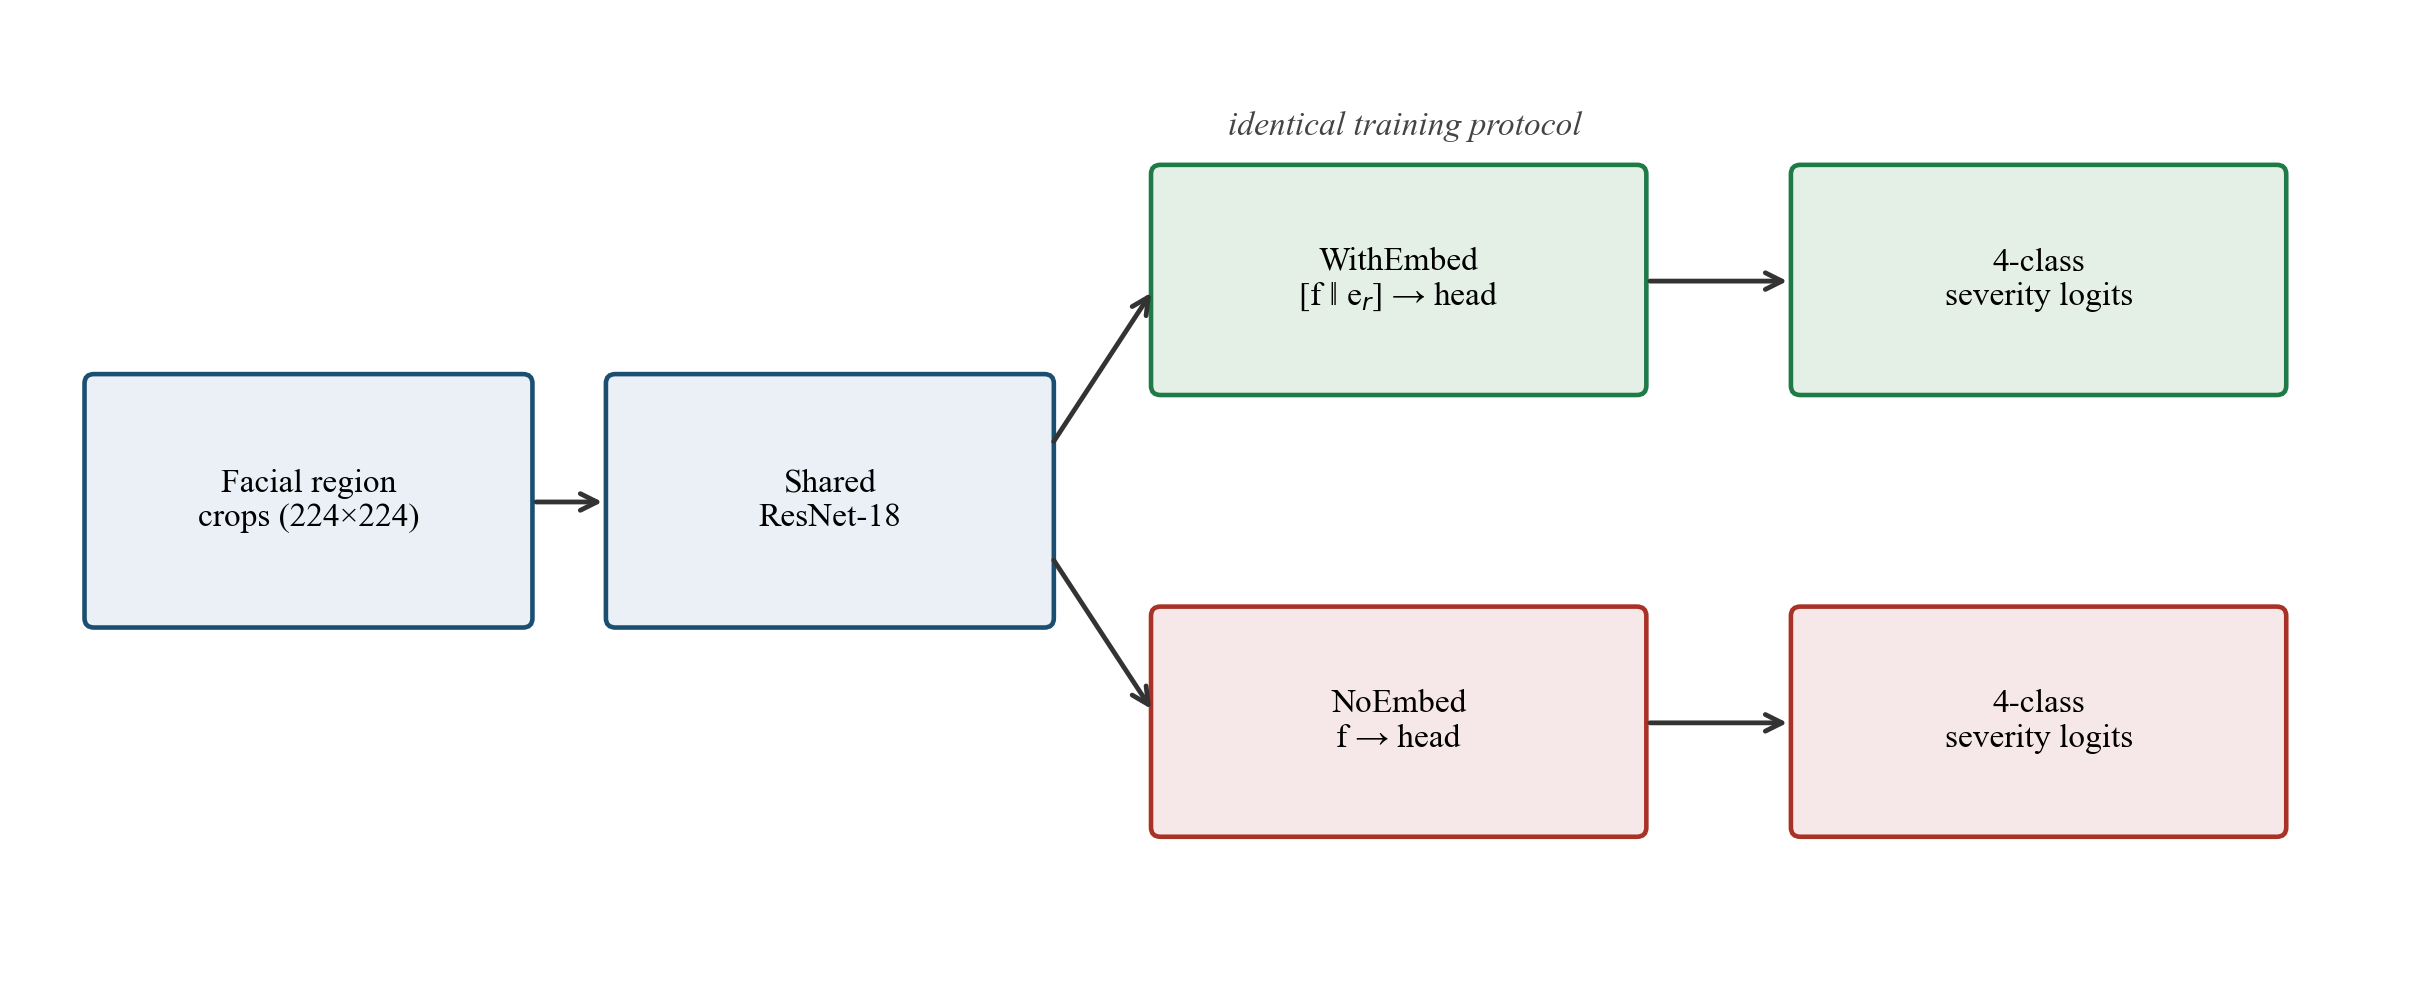
\includegraphics[width=0.92\columnwidth]{fig_ablation_pipeline.png}
\caption{Ablation design used in this study: shared convolutional backbone with anatomical embeddings (WithEmbed) versus the same backbone without them (NoEmbed).}
\label{fig:pipeline}
\end{figure}
\FloatBarrier

\begin{figure}[!htbp]
\centering
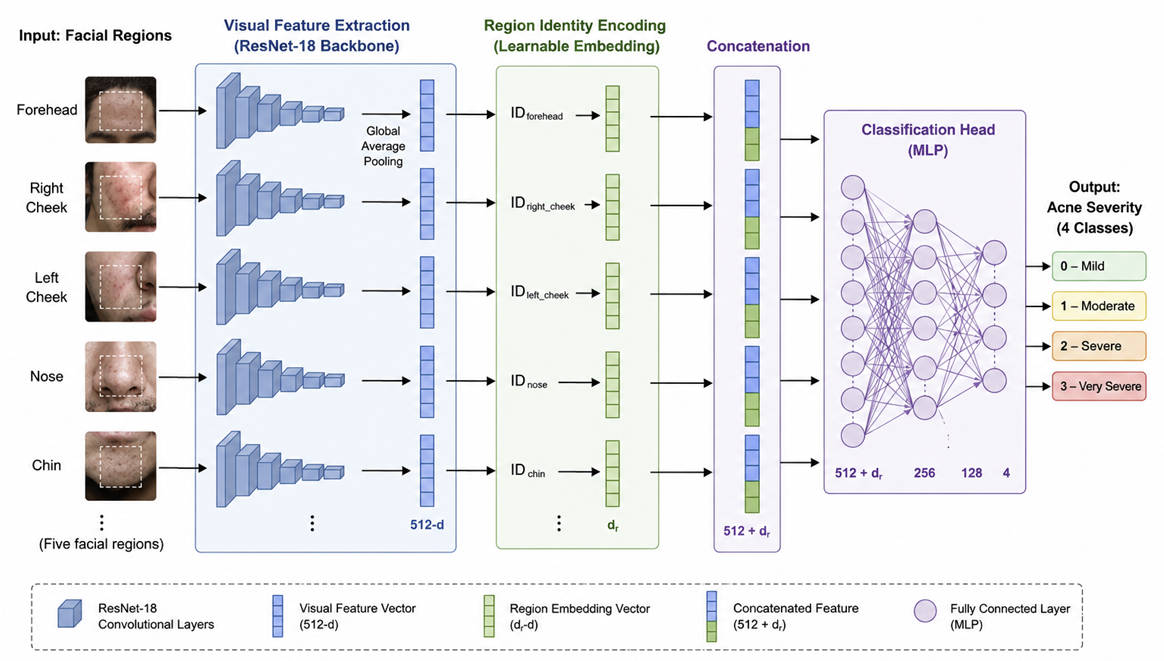
\includegraphics[width=0.88\columnwidth]{fig3_architecture.jpg}
\caption{WithEmbed network: convolutional features concatenated with a 64-dimensional region embedding before the classification head.}
\label{fig:arch}
\end{figure}
\FloatBarrier

\subsection{Training Protocol}
Optimization uses Adam \cite{kingma2015adam} with learning rate $10^{-4}$ and weighted cross-entropy. Class weights are estimated from the training histogram to reduce bias toward majority severity grades. The batch size is 16, the epoch budget is 40, the learning rate follows ReduceLROnPlateau, and training stops early after 10 epochs without improvement on a robustness-oriented monitor. Augmentation includes horizontal flips ($p=0.5$), rotations of $\pm25^\circ$, color jitter, Gaussian blur, and random erasing. Models are trained from scratch on the acne crops rather than from a large-scale natural-image checkpoint such as ImageNet \cite{deng2009imagenet}. Seed, split, and device are held fixed across compared runs.

The primary NoEmbed model is trained from scratch, which asks whether anatomical codes are needed to learn the task at all. A complementary transfer run copies the WithEmbed encoder weights into a NoEmbed network and continues training without embeddings. That setting probes whether features acquired under embedding supervision remain informative once the codes are dropped.

\subsection{Evaluation Metrics}
We report accuracy, weighted F1, and macro F1 on the clean test split, plus weighted F1 stratified by facial region. For WithEmbed we also compute pairwise cosine similarities among the five embedding vectors. Mild photometric and geometric perturbations are used only to guide checkpoint selection during training; the tables below refer to unperturbed evaluation.

\section{Experimental Results}
\subsection{Overall Ablation}
Table~\ref{tab:ablation} and Figure~\ref{fig:overall} summarize the main comparison. WithEmbed reaches 95.2\% accuracy and weighted F1 of 0.95. The from-scratch NoEmbed baseline stays near chance-to-moderate performance at 48.4\% accuracy and weighted F1 of 0.49. The absolute differences are $+46.8$~pp in accuracy and $+46.3$~pp in weighted F1. Under the protocol used here, removing anatomical conditioning leaves the shared backbone unable to exploit multi-region crops effectively.

\begin{table}[t]
\caption{Primary ablation on the held-out test set (1{,}090 crops).}
\label{tab:ablation}
\centering
\small
\begin{tabular}{lccc}
\toprule
Model & Acc. (\%) & F1$_w$ & F1$_{macro}$ \\
\midrule
NoEmbed (scratch) & 48.4 & 0.49 & 0.45 \\
WithEmbed & 95.2 & 0.95 & 0.95 \\
\midrule
$\Delta$ (With$-$No) & $+46.8$ & $+0.46$ & $+0.50$ \\
\bottomrule
\end{tabular}
\end{table}

\begin{figure}[!htbp]
\centering
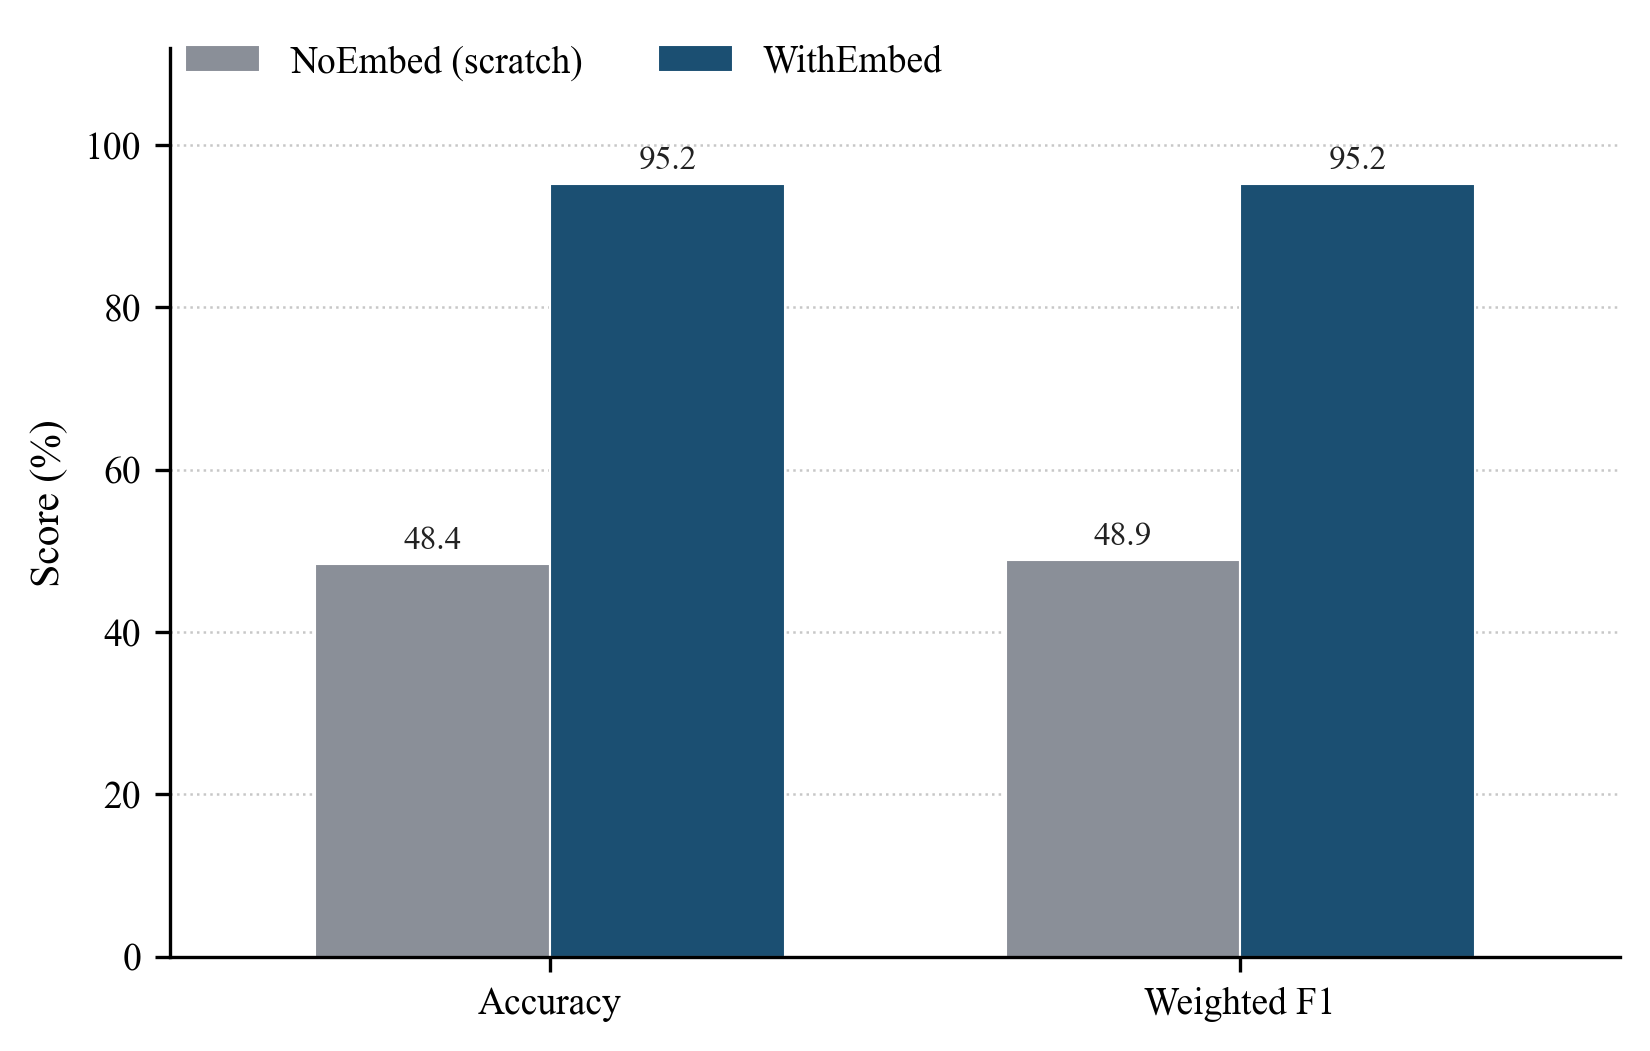
\includegraphics[width=0.82\columnwidth]{fig_ablation_overall.png}
\caption{Accuracy and weighted F1 (\%) for NoEmbed trained from scratch versus WithEmbed.}
\label{fig:overall}
\end{figure}
\FloatBarrier

\subsection{Region-wise Gains}
Figure~\ref{fig:region} and Table~\ref{tab:regions} break the same comparison down by anatomy. Every region benefits from embeddings. The largest weighted-F1 lifts appear on the right cheek ($+54.2$~pp) and chin ($+49.4$~pp), where illumination, facial hair, and lesion layout vary more. Forehead is comparatively easy for both models, but WithEmbed still raises F1 from 0.74 to 0.99 ($+24.7$~pp).

\begin{table}[t]
\caption{Weighted F1 by facial region.}
\label{tab:regions}
\centering
\small
\begin{tabular}{lcccc}
\toprule
Region & NoEmbed & WithEmbed & $\Delta$ (pp) & Sup. \\
\midrule
Forehead & 0.74 & 0.99 & $+24.7$ & 93 \\
Chin & 0.44 & 0.93 & $+49.4$ & 329 \\
Nose & 0.56 & 0.97 & $+41.2$ & 103 \\
L.\ cheek & 0.53 & 0.93 & $+40.4$ & 169 \\
R.\ cheek & 0.42 & 0.96 & $+54.2$ & 396 \\
\bottomrule
\end{tabular}
\end{table}

\begin{figure}[!htbp]
\centering
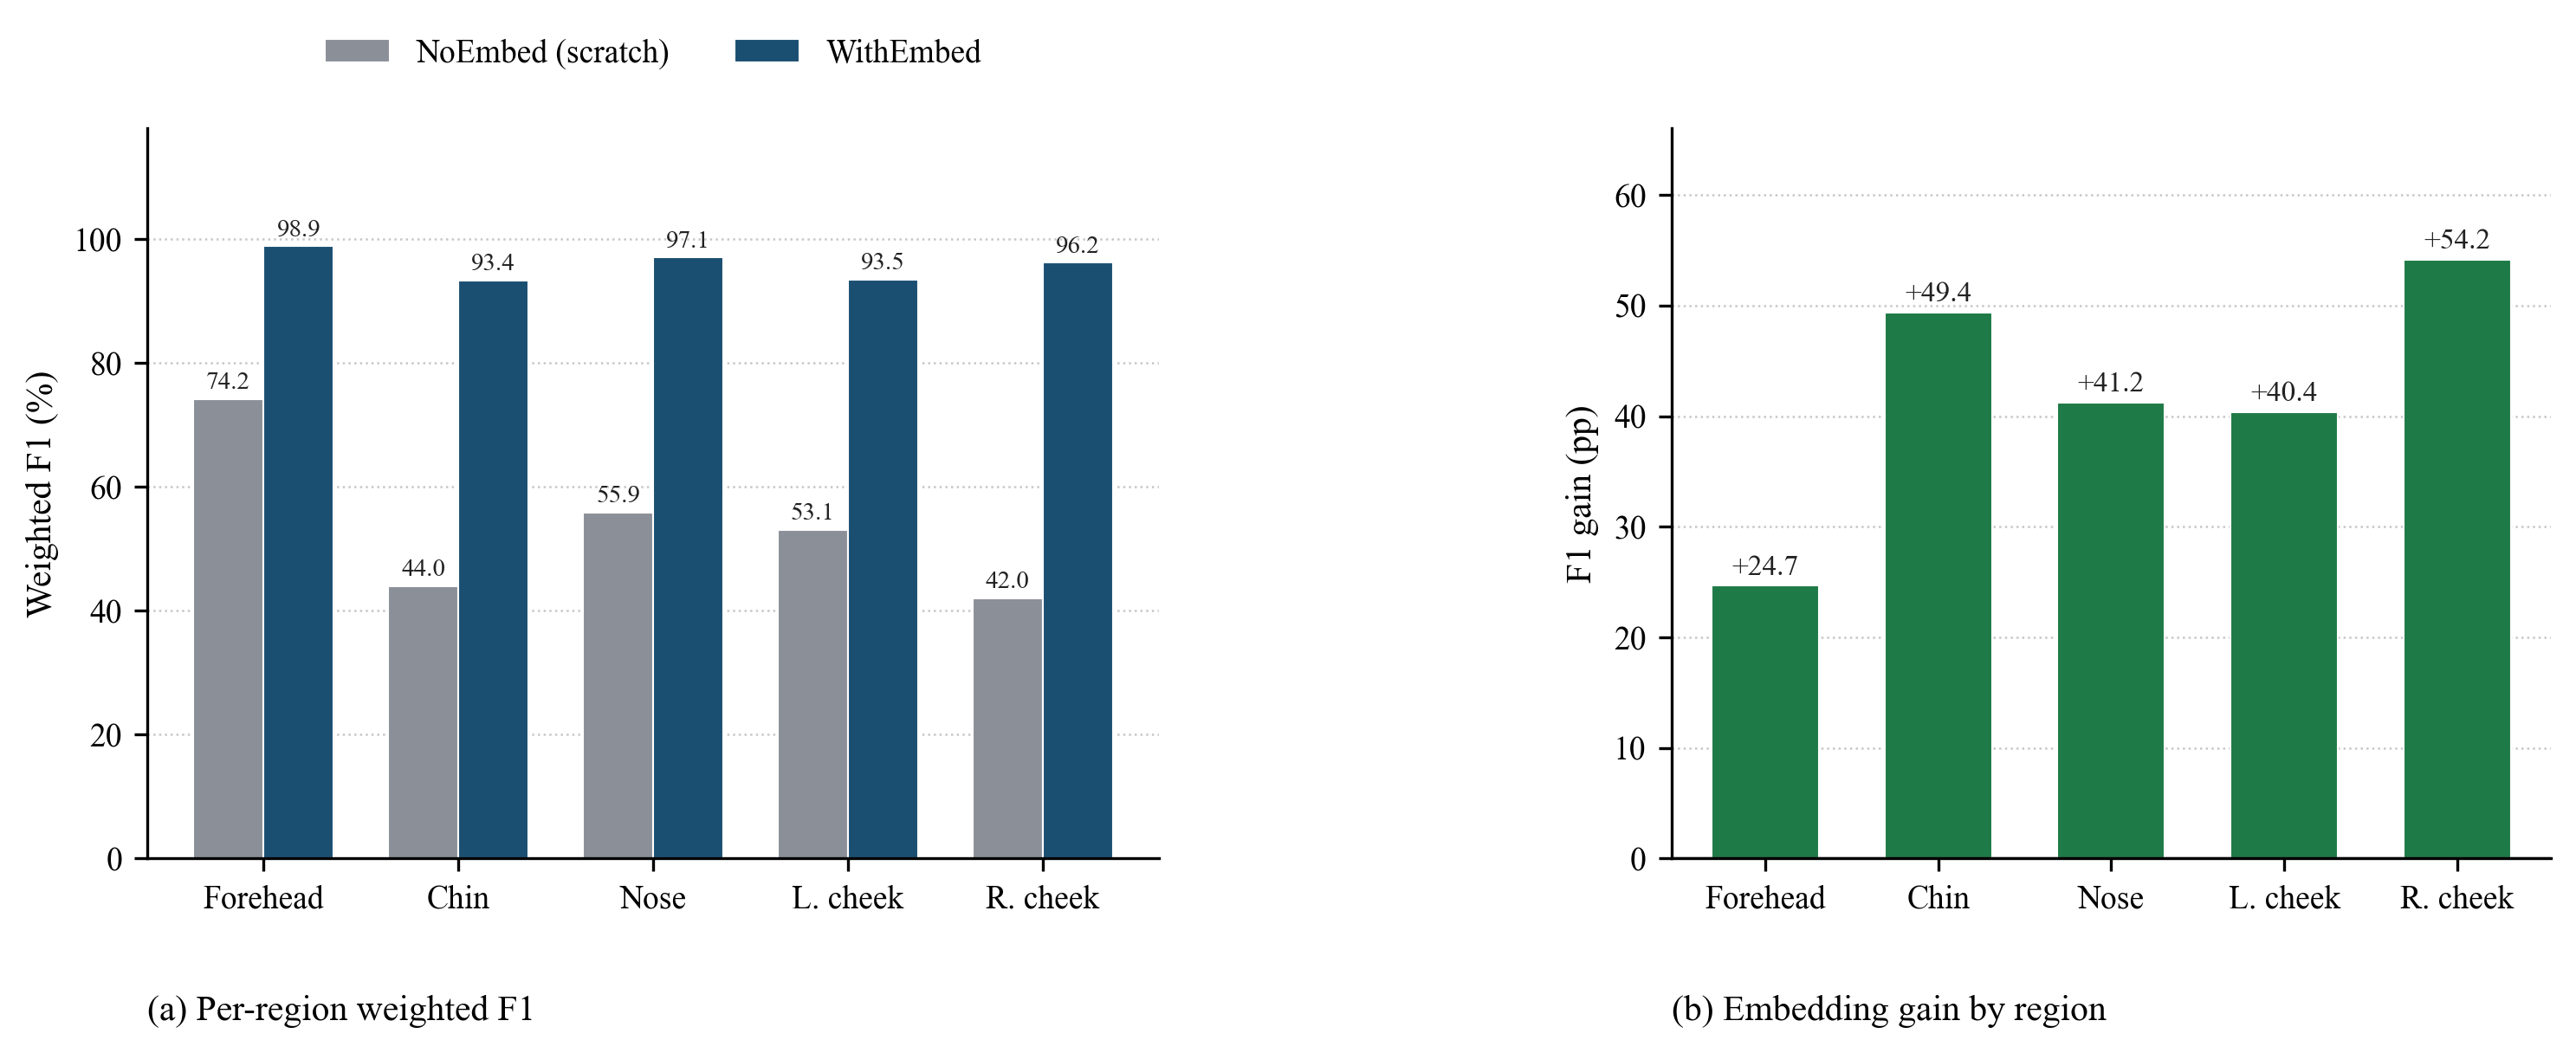
\includegraphics[width=0.95\columnwidth]{fig_ablation_by_region.png}
\caption{Per-region weighted F1 and the corresponding embedding-induced gain in percentage points.}
\label{fig:region}
\end{figure}
\FloatBarrier

\subsection{Embedding Geometry and Transfer Check}
Off-diagonal cosine similarities among the five embeddings are small (mean $0.04$; Figure~\ref{fig:sim}), so the codes do not collapse onto a single direction. In the transfer setting, NoEmbed warm-started from WithEmbed reaches 96.5\% accuracy. Features learned with anatomical supervision therefore remain useful even after the embedding layer is removed, which is consistent with embeddings acting mainly as a training-time inductive bias.

\begin{figure}[!htbp]
\centering
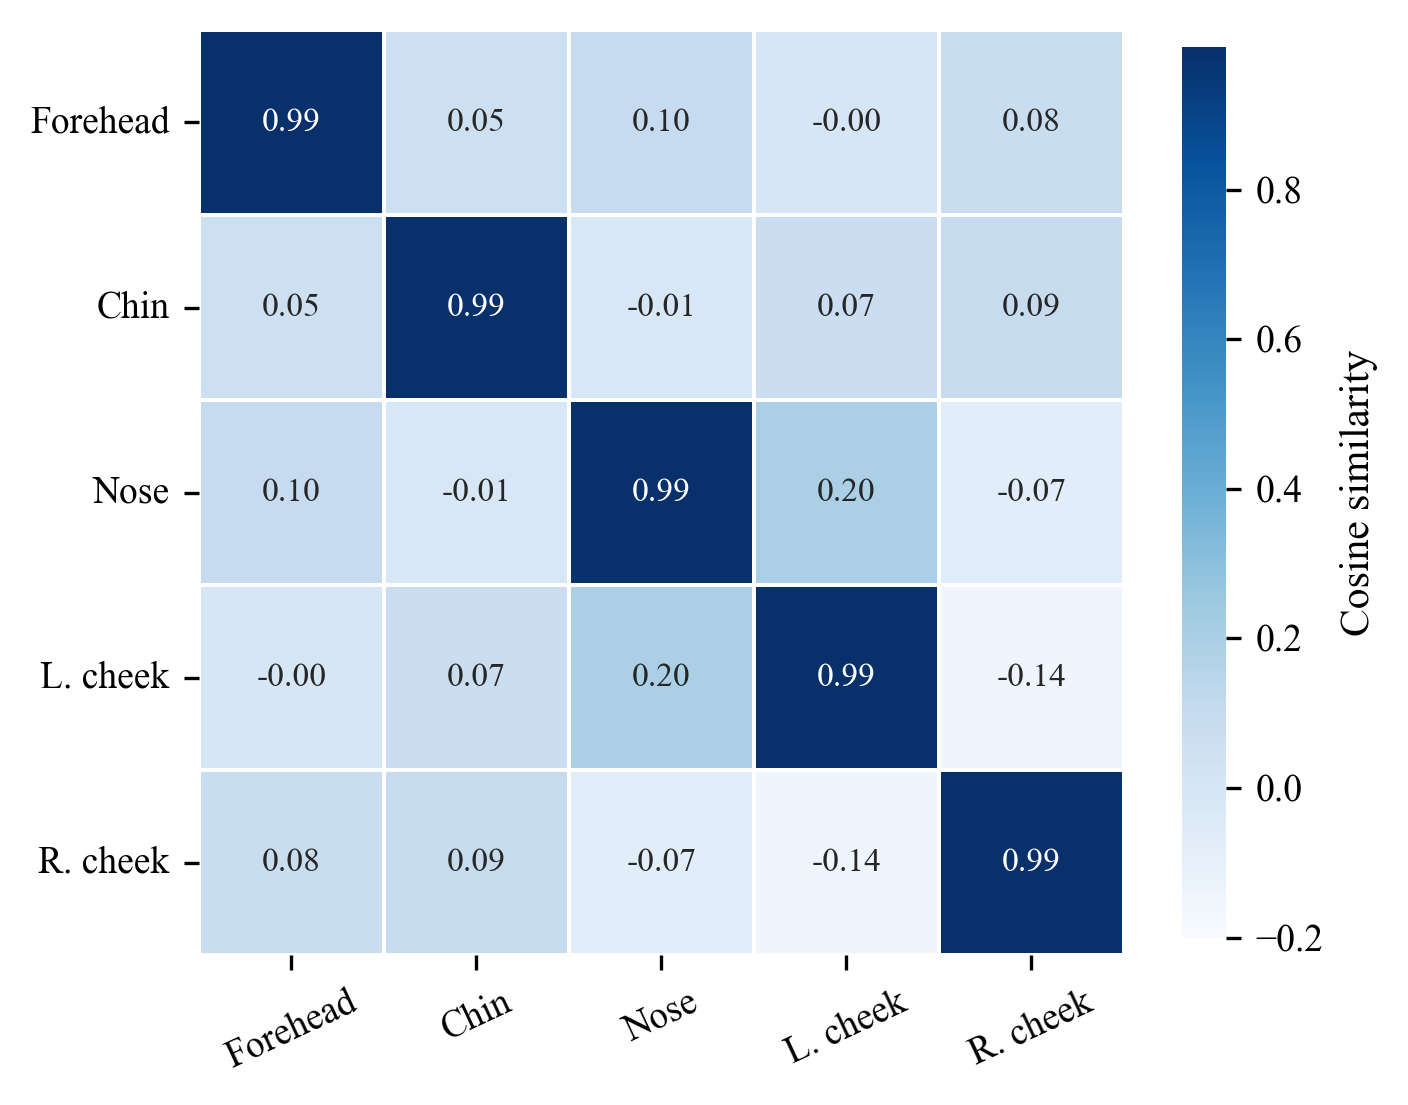
\includegraphics[width=0.72\columnwidth]{fig_embedding_similarity.png}
\caption{Pairwise cosine similarity of the five learned anatomical embeddings.}
\label{fig:sim}
\end{figure}
\FloatBarrier

\subsection{Mobile Feasibility Sketch}
The ablation remains the main contribution. Figure~\ref{fig:app} only outlines a possible surrounding workflow (capture, region extraction, classification, and longitudinal reporting). It is included to show that the classifier could sit in a lightweight decision-support pipeline, not to claim a finished clinical product. Usability testing and prospective evaluation with clinicians are left for future work.

\begin{figure}[!htbp]
\centering
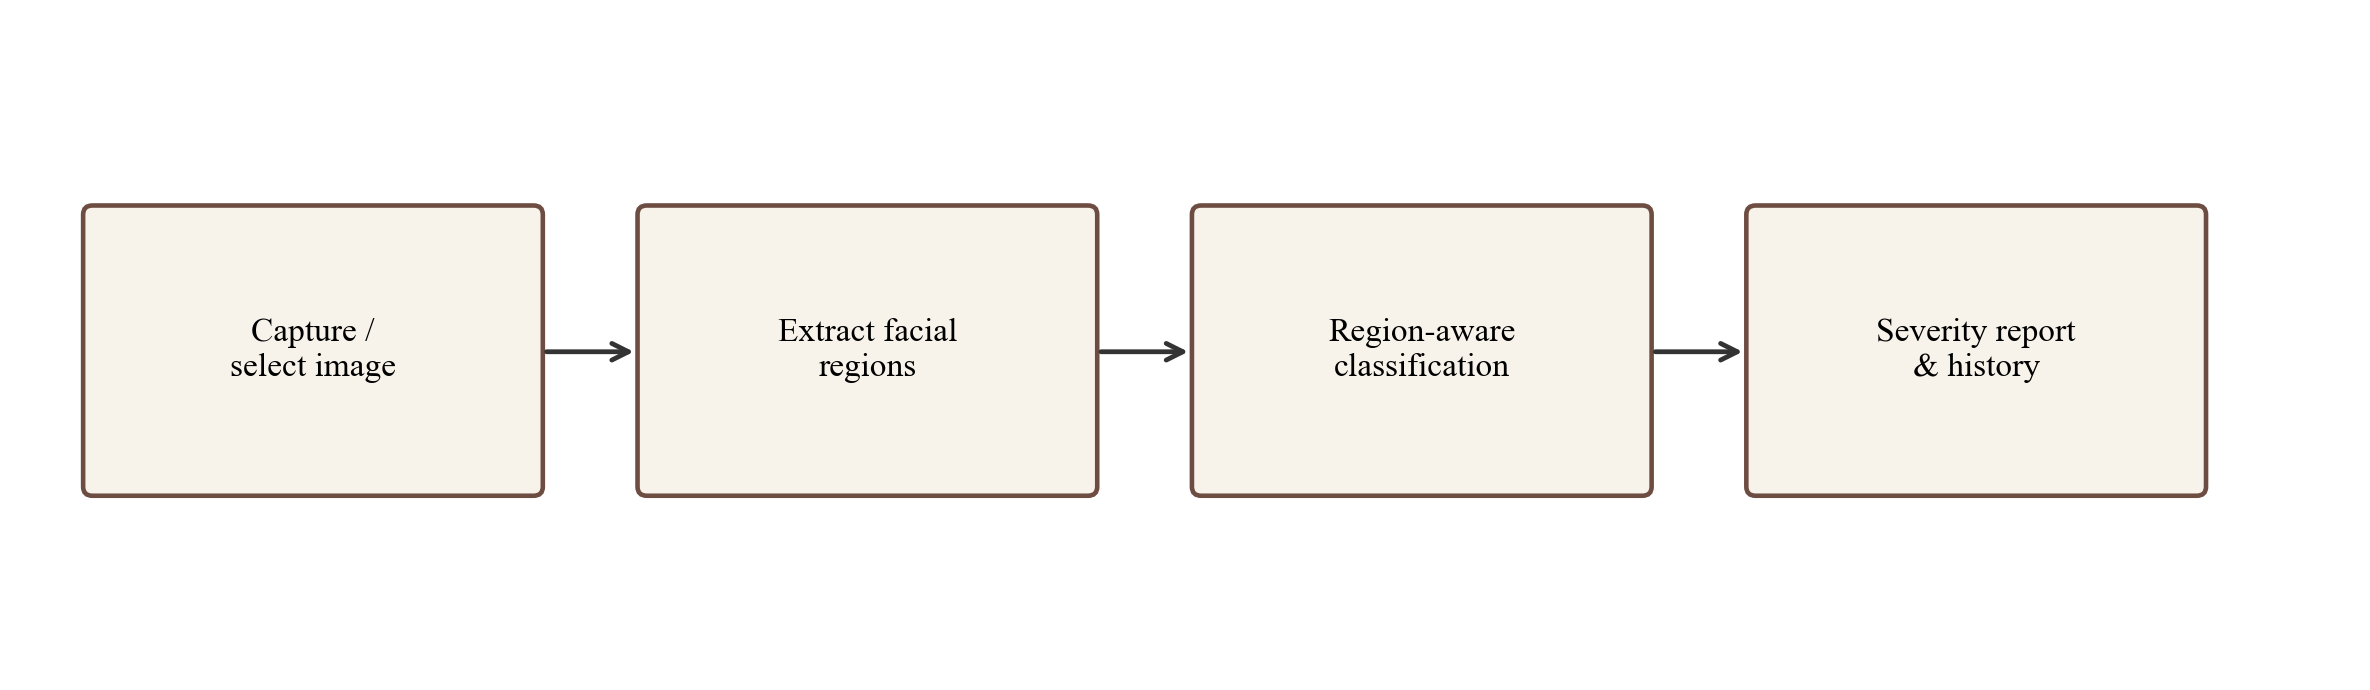
\includegraphics[width=0.92\columnwidth]{fig_app_concept.png}
\caption{Conceptual mobile workflow in which the region-aware classifier could be embedded.}
\label{fig:app}
\end{figure}
\FloatBarrier

\section{Discussion and Limitations}
The from-scratch ablation indicates that anatomical embeddings matter when a single ResNet-18 must learn from heterogeneous facial zones. Without region identity, the encoder has to absorb zone-dependent appearance into one representation; in our runs that strategy did not succeed. Adding a low-dimensional embedding restores strong test performance and yields the largest gains where visual variability is higher (cheeks and chin).

The transfer result adds nuance. Once the backbone has been shaped under embedding supervision, a NoEmbed head can still score 96.5\%. We therefore do not claim that embeddings must remain present at inference in every deployment. A more cautious reading is that they help the shared encoder organize region-dependent cues during learning, after which much of that structure may already reside in the convolutional features.

Several limits should be kept in view. The study uses two public datasets with incomplete control over patient identity across splits. Labels describe region severity rather than individual lesions. Softmax probabilities are uncalibrated, and the mobile sketch has not been evaluated with clinicians or patients. Broader phototype coverage and device diversity are still required before any clinical recommendation.

\section{Conclusion}
This work isolated the contribution of learnable anatomical embeddings in a shared convolutional backbone for four-level facial acne severity classification. Under a matched protocol, WithEmbed raised accuracy from 48.4\% to 95.2\% ($+46.8$~pp) and weighted F1 from 0.49 to 0.95 ($+46.3$~pp) relative to NoEmbed trained from scratch. Gains appeared in every facial region and were largest on the cheeks and chin, where appearance varies more across patients and acquisition conditions.

The embedding analysis and the transfer experiment refine that finding. Cosine similarities among region codes remained low, which indicates that the model did not collapse all zones onto a single direction. At the same time, a NoEmbed network warm-started from WithEmbed still reached 96.5\% accuracy. Anatomical conditioning therefore looks most useful as a learning signal that helps the encoder organize region-dependent cues; once those features exist, the explicit codes are not always required at inference.

Several caveats remain. The study relies on public image collections without guaranteed patient-level separation, uses region-level rather than lesion-level labels, and does not calibrate Softmax confidence. The mobile workflow is only a conceptual sketch. Even with those limits, the ablation supports a practical design choice: for multi-region acne grading with a shared backbone, a low-dimensional anatomical embedding is a small change that can produce a large improvement during training. Future work should prioritize external validation, probability calibration, and a carefully scoped evaluation of decision-support use.

\begin{thebibliography}{99}
\bibitem{zaenglein2018acne}
A.~L. Zaenglein, ``Acne vulgaris,'' \emph{New England Journal of Medicine}, vol. 379, no. 14, pp. 1343--1352, 2018.

\bibitem{vallerand2018risk}
I.~A. Vallerand \emph{et al.}, ``Risk of depression among patients with acne in the UK,'' \emph{Brit. J. Dermatol.}, vol. 178, no. 3, pp. e194--e195, 2018.

\bibitem{hayashi2008grading}
N.~Hayashi \emph{et al.}, ``Development of a new acne severity grading system,'' \emph{J. Dermatol.}, vol. 35, no. 5, pp. 255--260, 2008.

\bibitem{bhate2013epi}
K.~Bhate and H.~C. Williams, ``Epidemiology of acne vulgaris,'' \emph{Brit. J. Dermatol.}, vol. 168, no. 3, pp. 474--485, 2013.

\bibitem{moreno2017teledermatology}
D.~Moreno-Ram{\'i}rez and G.~Argenziano, ``Teledermatology and mobile applications in the management of patients with skin lesions,'' \emph{Acta Dermato-Venereologica}, vol. 97, no. 4, pp. 412--418, 2017.

\bibitem{tran2011mobile}
K.~Tran \emph{et al.}, ``Mobile teledermatology in the developing world: using a store-and-forward system for diagnosis and follow-up,'' \emph{J. Amer. Acad. Dermatol.}, vol. 64, no. 2, pp. 302--309, 2011.

\bibitem{shen2018acne}
X.~Shen \emph{et al.}, ``An automatic diagnosis method of facial acne vulgaris based on convolutional neural network,'' \emph{Scientific Reports}, vol. 8, Art. no. 5839, 2018.

\bibitem{wu2019joint}
X.~Wu \emph{et al.}, ``Joint acne image grading and counting via label distribution learning,'' in \emph{Proc. IEEE/CVF ICCV}, 2019, pp. 10642--10651.

\bibitem{nasr2016melanoma}
E.~Nasr-Esfahani \emph{et al.}, ``Melanoma detection by analysis of clinical images using convolutional neural network,'' in \emph{Proc. IEEE EMBC}, 2016, pp. 1373--1376.

\bibitem{brinker2019cnn}
T.~J. Brinker \emph{et al.}, ``A convolutional neural network trained with dermoscopic images performed on par with 145 dermatologists in a clinical melanoma image classification task,'' \emph{Eur. J. Cancer}, vol. 111, pp. 148--154, 2019.

\bibitem{esteva2017dermatologist}
A.~Esteva \emph{et al.}, ``Dermatologist-level classification of skin cancer with deep neural networks,'' \emph{Nature}, vol. 542, pp. 115--118, 2017.

\bibitem{tschandl2018ham10000}
P.~Tschandl, C.~Rosendahl, and H.~Kittler, ``The HAM10000 dataset, a large collection of multi-source dermatoscopic images of common pigmented skin lesions,'' \emph{Scientific Data}, vol. 5, Art. no. 180161, 2018.

\bibitem{codella2018isic}
N.~C.~F. Codella \emph{et al.}, ``Skin lesion analysis toward melanoma detection: A challenge at the 2017 International Symposium on Biomedical Imaging (ISBI), hosted by the International Skin Imaging Collaboration (ISIC),'' in \emph{Proc. IEEE ISBI}, 2018, pp. 168--172.

\bibitem{junayed2020acnenet}
M.~S. Junayed \emph{et al.}, ``AcneNet---A deep CNN based classification approach for acne classes,'' in \emph{Proc. ICIT}, 2020, pp. 203--208.

\bibitem{thiboutot2009global}
D.~Thiboutot \emph{et al.}, ``New insights into the management of acne: An update from the Global Alliance to Improve Outcomes in Acne Group,'' \emph{J. Amer. Acad. Dermatol.}, vol. 60, no. 5, pp. S1--S50, 2009.

\bibitem{seite2019digital}
S.~Seit{\'e} \emph{et al.}, ``Development and accuracy of an artificial intelligence algorithm for acne grading from smartphone photographs,'' \emph{Experimental Dermatology}, vol. 28, no. 12, pp. 1454--1459, 2019.

\bibitem{sandler2018mobilenetv2}
M.~Sandler \emph{et al.}, ``MobileNetV2: Inverted residuals and linear bottlenecks,'' in \emph{Proc. IEEE/CVF CVPR}, 2018, pp. 4510--4520.

\bibitem{tan2019efficientnet}
M.~Tan and Q.~V. Le, ``EfficientNet: Rethinking model scaling for convolutional neural networks,'' in \emph{Proc. ICML}, 2019, pp. 6105--6114.

\bibitem{huang2017densenet}
G.~Huang, Z.~Liu, L.~van~der~Maaten, and K.~Q. Weinberger, ``Densely connected convolutional networks,'' in \emph{Proc. IEEE CVPR}, 2017, pp. 4700--4708.

\bibitem{redmon2017yolo9000}
J.~Redmon and A.~Farhadi, ``YOLO9000: Better, faster, stronger,'' in \emph{Proc. IEEE CVPR}, 2017, pp. 7263--7271.

\bibitem{dosovitskiy2021vit}
A.~Dosovitskiy \emph{et al.}, ``An image is worth 16x16 words: Transformers for image recognition at scale,'' in \emph{Proc. ICLR}, 2021.

\bibitem{selvaraju2017gradcam}
R.~R. Selvaraju \emph{et al.}, ``Grad-CAM: Visual explanations from deep networks via gradient-based localization,'' in \emph{Proc. IEEE ICCV}, 2017, pp. 618--626.

\bibitem{byamba2015mobile}
K.~Byamba \emph{et al.}, ``Mobile teledermatology for a prompter and more efficient dermatological care in rural Mongolia,'' \emph{Brit. J. Dermatol.}, vol. 173, no. 1, pp. 265--267, 2015.

\bibitem{minagawa2021aiacne}
A.~Minagawa, H.~Koga, and R.~Okuyama, ``Artificial intelligence for the classification of acne severity from clinical photographs,'' \emph{J. Dermatol.}, vol. 48, no. 7, pp. e321--e322, 2021.

\bibitem{kingma2015adam}
D.~P. Kingma and J.~Ba, ``Adam: A method for stochastic optimization,'' in \emph{Proc. ICLR}, 2015.

\bibitem{srivastava2014dropout}
N.~Srivastava \emph{et al.}, ``Dropout: A simple way to prevent neural networks from overfitting,'' \emph{J. Mach. Learn. Res.}, vol. 15, pp. 1929--1958, 2014.

\bibitem{ioffe2015batchnorm}
S.~Ioffe and C.~Szegedy, ``Batch normalization: Accelerating deep network training by reducing internal covariate shift,'' in \emph{Proc. ICML}, 2015, pp. 448--456.

\bibitem{deng2009imagenet}
J.~Deng \emph{et al.}, ``ImageNet: A large-scale hierarchical image database,'' in \emph{Proc. IEEE CVPR}, 2009, pp. 248--255.
\end{thebibliography}

\end{document}
